\documentclass[11pt,a4paper]{article}

\usepackage[utf8]{inputenc}
\usepackage[T1]{fontenc}
\usepackage{geometry}
\usepackage{booktabs}
\usepackage{longtable}
\usepackage{array}
\usepackage{hyperref}
\usepackage{xcolor}
\usepackage{listings}
\usepackage{tikz}
\usepackage{caption}
\usepackage{enumitem}
\usetikzlibrary{arrows.meta, positioning, shapes.geometric}

\geometry{margin=2.5cm}

\definecolor{codebg}{RGB}{245,245,245}
\definecolor{codegray}{RGB}{110,110,110}

\lstset{
  basicstyle=\ttfamily\small,
  backgroundcolor=\color{codebg},
  breaklines=true,
  frame=single,
  framesep=4pt,
  rulecolor=\color{codegray},
  columns=fullflexible,
  showstringspaces=false
}

\hypersetup{
  colorlinks=true,
  linkcolor=black,
  urlcolor=blue,
  citecolor=black,
  pdftitle={Relatorio Tecnico - Agente de IA para Triagem de Logs de Seguranca},
  pdfauthor={cenourin}
}

\title{\textbf{Relatório Técnico}\\[4pt]
\large Agente de IA para Triagem de Logs de Segurança}
\author{cenourin \\ \small Portfólio técnico --- IA aplicada a Cibersegurança}
\date{15 de julho de 2026}

\begin{document}

\maketitle

\begin{abstract}
\noindent Este documento descreve, de forma consolidada, os requisitos, a arquitetura,
o modelo de dados, o plano e a execução de testes, a análise dos resultados obtidos e
uma proposta de aplicação em cenário real do \emph{Agente de IA para Triagem de Logs de
Segurança}. O sistema classifica eventos de log (SSH, firewall, EDR) em
\texttt{SUSPEITO}, \texttt{NORMAL} ou \texttt{CRITICO}, gera um resumo em linguagem
natural e sugere uma ação de resposta, utilizando um modelo de linguagem (LLM) quando
disponível ou um classificador heurístico determinístico como alternativa local.
\end{abstract}

\tableofcontents

% =====================================================================
\section{Introdução e contexto}
% =====================================================================

O projeto foi motivado pelo interesse pessoal em aplicar modelos de IA para apoiar
análises e a criação de agentes de IA para operações de segurança. O objetivo é
demonstrar, em escala reduzida porém funcional, um componente
típico de triagem automatizada de alertas em um SOC (\emph{Security Operations Center}):
receber um evento de log bruto, decidir se ele é relevante, explicar o porquê em
linguagem natural e sugerir a próxima ação para um analista humano.

O sistema foi construído com duas premissas centrais de engenharia:

\begin{enumerate}
  \item \textbf{Disponibilidade sem dependência externa obrigatória}: o serviço deve
  funcionar integralmente sem exigir uma chave de API paga, para ser demonstrável e
  testável por qualquer avaliador.
  \item \textbf{Determinismo em testes}: a suíte automatizada não deve depender de rede
  nem de credenciais, para ser executável em qualquer ambiente (incluindo integração
  contínua).
\end{enumerate}

Essas premissas motivaram a decisão de arquitetura central do projeto, descrita na
Seção~\ref{sec:arquitetura}: um motor duplo de classificação (LLM real e heurística
local), com seleção automática e \emph{fallback} transparente.

% =====================================================================
\section{Documento de requisitos}
% =====================================================================

\subsection{Escopo}

\textbf{Dentro do escopo:} ingestão de logs em texto (arquivo ou requisição HTTP, um
evento por linha); classificação em três níveis; geração de resumo em linguagem
natural; sugestão de ação; persistência dos eventos processados e consulta posterior
via API; seleção automática entre modo real (LLM via API Anthropic) e modo heurístico
local.

\textbf{Fora do escopo:} coleta de logs em produção (agentes de coleta, Syslog,
Filebeat etc.); execução automática de bloqueios em firewall real (a ação é apenas
\emph{sugerida}); interface gráfica além da documentação interativa gerada
automaticamente pelo FastAPI (Swagger/OpenAPI).

\subsection{Atores}

\begin{itemize}[nosep]
  \item \textbf{Analista de SOC} --- consome os alertas triados via API para
  priorizar investigação.
  \item \textbf{Sistema de ingestão} (simulado) --- arquivo de log ou chamada HTTP
  que alimenta o agente.
  \item \textbf{Provedor de LLM} (Anthropic Claude) --- opcional, usado quando a
  variável \verb|ANTHROPIC_API_KEY| está configurada.
\end{itemize}

\subsection{Requisitos funcionais}

\begin{longtable}{p{1.4cm}p{10.5cm}p{1.6cm}}
\toprule
\textbf{ID} & \textbf{Descrição} & \textbf{Prioridade} \\
\midrule
\endhead
RF01 & Receber uma linha de log via \verb|POST /events/analyze| e retornar classificação, resumo e ação sugerida. & Alta \\
RF02 & Processar um lote de logs via \verb|POST /events/analyze-batch|. & Alta \\
RF03 & Processar um arquivo de log completo via CLI (\verb|python -m app.cli --file <path>|). & Alta \\
RF04 & Persistir cada evento processado (log original, classificação, resumo, ação, timestamp) em banco SQLite. & Alta \\
RF05 & Expor \verb|GET /events| para listar eventos processados, com filtro opcional por classificação. & Média \\
RF06 & Expor \verb|GET /events/{id}| para detalhar um evento específico. & Média \\
RF07 & Expor \verb|GET /health| para checagem de disponibilidade. & Alta \\
RF08 & Sem \verb|ANTHROPIC_API_KEY|, usar classificador heurístico local sem falhar. & Alta \\
RF09 & Com \verb|ANTHROPIC_API_KEY|, usar o modelo Claude para classificar e resumir o evento. & Média \\
RF10 & Disponibilizar dados de exemplo (\verb|data/sample_logs.log|) prontos para demonstração. & Baixa \\
RF11 & Expor \verb|GET /events/stats| com contagem de eventos por classificação. & Baixa \\
\bottomrule
\caption{Requisitos funcionais}
\end{longtable}

\subsection{Requisitos não funcionais}

\begin{longtable}{p{1.6cm}p{12cm}}
\toprule
\textbf{ID} & \textbf{Descrição} \\
\midrule
\endhead
RNF01 & O serviço deve subir integralmente via \verb|docker compose up| sem configuração manual adicional. \\
RNF02 & \verb|GET /health| deve responder em menos de 200\,ms em ambiente local. \\
RNF03 & Cobertura de testes automatizados para o classificador heurístico e para os principais endpoints da API. \\
RNF04 & Nenhuma credencial versionada em texto puro; configuração via variáveis de ambiente (\verb|.env|, não commitado). \\
RNF05 & Degradação previsível (modo heurístico) caso o provedor de LLM esteja indisponível; nunca retornar erro 500 por esse motivo. \\
RNF06 & Logs da aplicação legíveis via \verb|docker compose logs|. \\
\bottomrule
\caption{Requisitos não funcionais}
\end{longtable}

\subsection{Casos de uso}

\textbf{UC01 --- Analisar evento único.} Cliente envia \verb|POST /events/analyze|;
o sistema seleciona o motor de classificação, classifica, resume, sugere ação,
persiste e retorna o resultado.

\textbf{UC02 --- Processar arquivo de logs em lote (CLI).} Operador executa
\verb|python -m app.cli --file data/sample_logs.log|; o sistema aplica UC01 a cada
linha e imprime um resumo tabular no terminal.

\textbf{UC03 --- Consultar histórico de eventos.} Analista chama
\verb|GET /events?classification=SUSPEITO| e recebe a lista filtrada, mais recentes
primeiro.

\subsection{Critérios de aceite}

\begin{itemize}[nosep]
  \item \verb|docker compose up --build| inicia a API na porta \texttt{8001} sem erros.
  \item \verb|curl http://localhost:8001/health| retorna \texttt{200 OK}.
  \item Um log de força bruta SSH conhecido retorna classificação \texttt{SUSPEITO}
  ou \texttt{CRITICO} com ação sugerida não vazia, tanto em modo heurístico quanto em
  modo LLM.
  \item \texttt{pytest} roda com sucesso dentro do container.
\end{itemize}

% =====================================================================
\section{Arquitetura e engenharia de software}
\label{sec:arquitetura}
% =====================================================================

\subsection{Visão geral}

\begin{center}
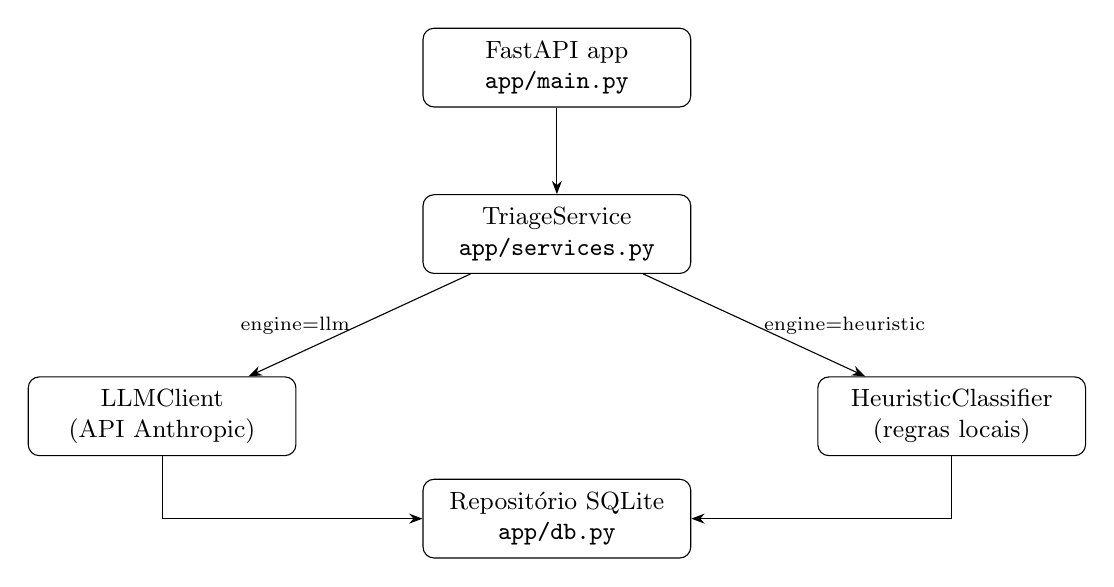
\begin{tikzpicture}[
  block/.style={rectangle, draw, rounded corners, minimum width=3.4cm, minimum height=1cm, align=center, font=\small},
  >=Stealth
]
\node[block] (api) {FastAPI app\\\texttt{app/main.py}};
\node[block, below=1.1cm of api] (service) {TriageService\\\texttt{app/services.py}};
\node[block, below left=1.3cm and 1.6cm of service] (llm) {LLMClient\\(API Anthropic)};
\node[block, below right=1.3cm and 1.6cm of service] (heur) {HeuristicClassifier\\(regras locais)};
\node[block, below=2.6cm of service] (db) {Repositório SQLite\\\texttt{app/db.py}};

\draw[->] (api) -- (service);
\draw[->] (service) -- node[left, font=\scriptsize] {engine=llm} (llm);
\draw[->] (service) -- node[right, font=\scriptsize] {engine=heuristic} (heur);
\draw[->] (llm) |- (db);
\draw[->] (heur) |- (db);
\end{tikzpicture}
\captionof{figure}{Visão geral da arquitetura: a API delega ao \texttt{TriageService},
que escolhe o motor de classificação e persiste o resultado.}
\end{center}

O CLI (\texttt{app/cli.py}) reutiliza o mesmo \texttt{TriageService}, garantindo que a
lógica de classificação seja única independentemente do canal de entrada.

\subsection{Módulos}

\begin{longtable}{p{3.6cm}p{9.5cm}}
\toprule
\textbf{Módulo} & \textbf{Responsabilidade} \\
\midrule
\endhead
\texttt{app/main.py} & Definição da API FastAPI, rotas e serialização HTTP. \\
\texttt{app/services.py} & \texttt{TriageService}: orquestra escolha de engine, chama classificador e persiste resultado. \\
\texttt{app/llm\_client.py} & Cliente do LLM (Anthropic Claude): constrói o prompt, chama a API, faz parsing da resposta estruturada (JSON). \\
\texttt{app/heuristics.py} & Classificador baseado em regras/regex para padrões comuns de logs de segurança. \\
\texttt{app/db.py} & Acesso a dados via SQLite (\texttt{sqlite3} da stdlib), schema e CRUD de eventos. \\
\texttt{app/models.py} & Modelos Pydantic (schemas de request/response) e dataclasses internas. \\
\texttt{app/cli.py} & Interface de linha de comando para processar arquivos de log em lote. \\
\texttt{app/config.py} & Leitura de variáveis de ambiente. \\
\bottomrule
\caption{Módulos do sistema e responsabilidades}
\end{longtable}

\subsection{Decisão de arquitetura: motor duplo (LLM + heurístico)}

\textbf{Contexto.} O objetivo do projeto é usar LLMs para apoiar triagem, mas o sistema
precisa permanecer demonstrável e testável sem exigir que quem avalie o portfólio
configure uma chave de API paga.

\textbf{Decisão.} \texttt{TriageService} seleciona o motor em tempo de execução: se
\verb|ANTHROPIC_API_KEY| estiver presente, usa \texttt{LLMClient} (chamada real ao
modelo Claude, configurável via \verb|ANTHROPIC_MODEL|); caso contrário, usa
\texttt{HeuristicClassifier}, que aplica expressões regulares para padrões conhecidos
(tentativas de autenticação falhas, port scan, malware/exploração, bloqueios de
firewall). Ambos os motores implementam a mesma interface de saída
(\texttt{ClassificationResult}), tornando a troca transparente para quem consome a API
--- o campo \texttt{engine} da resposta indica qual foi usado.

\textbf{Consequência.} O sistema é 100\% demonstrável offline e sem custo, e passa a
usar IA real assim que uma chave é adicionada ao \texttt{.env}, sem alteração de
código. O custo dessa decisão é discutido na análise de resultados
(Seção~\ref{sec:resultados}): a cobertura de testes automatizados do caminho real do
LLM é necessariamente baixa, pois os testes não têm credenciais.

\subsection{Tratamento de erros e resiliência}

Falha na chamada ao LLM (timeout, \emph{rate limit}, resposta malformada) é capturada
em \texttt{LLMClient} e aciona \emph{fallback} automático para
\texttt{HeuristicClassifier} \emph{naquela requisição específica}, registrando
\texttt{engine = "heuristic\_fallback"}. Isso atende ao RNF05: o serviço nunca retorna
500 ao usuário final por indisponibilidade do provedor externo. Uma linha de log vazia
é rejeitada com \texttt{422 Unprocessable Entity} por validação Pydantic (RF08 e
contrato de entrada).

\subsection{Modelo de dados}

Tabela \texttt{events} (SQLite):

\begin{longtable}{p{2.8cm}p{2.2cm}p{7.5cm}}
\toprule
\textbf{Coluna} & \textbf{Tipo} & \textbf{Descrição} \\
\midrule
\endhead
\texttt{id} & INTEGER PK & Identificador autoincremental \\
\texttt{log\_line} & TEXT & Linha de log original \\
\texttt{classification} & TEXT & \texttt{SUSPEITO} / \texttt{NORMAL} / \texttt{CRITICO} \\
\texttt{summary} & TEXT & Resumo em linguagem natural \\
\texttt{suggested\_action} & TEXT & \texttt{bloquear\_ip} / \texttt{investigar\_usuario} / \texttt{ignorar} / \texttt{escalar} \\
\texttt{engine} & TEXT & \texttt{llm} / \texttt{heuristic} / \texttt{heuristic\_fallback} \\
\texttt{created\_at} & TEXT (ISO 8601) & Timestamp de processamento \\
\bottomrule
\caption{Esquema da tabela \texttt{events}}
\end{longtable}

\subsection{Contrato da API (resumo)}

\begin{lstlisting}
POST /events/analyze
// request
{ "log_line": "Failed password for root from 203.0.113.9 port 51321 ssh2" }

// response 200
{
  "id": 1,
  "classification": "SUSPEITO",
  "summary": "Tentativa de login falhou para o usuario 'root' a partir do IP 203.0.113.9.",
  "suggested_action": "bloquear_ip",
  "engine": "heuristic",
  "created_at": "2026-07-15T12:00:00"
}
\end{lstlisting}

\texttt{GET /events?classification=SUSPEITO} retorna uma lista de eventos no mesmo
formato; \texttt{GET /events/stats} retorna
\texttt{\{"SUSPEITO": 3, "NORMAL": 10, "CRITICO": 1\}}.

\subsection{Empacotamento e execução}

Imagem baseada em \texttt{python:3.12-slim}; dependências mínimas
(\texttt{fastapi}, \texttt{uvicorn}, \texttt{pydantic}, \texttt{anthropic},
\texttt{pytest}, \texttt{httpx}). O \texttt{docker-compose.yml} expõe a porta
\texttt{8001}, monta \texttt{./data} como volume somente leitura (dados de exemplo) e
um volume nomeado para persistir o SQLite entre reinícios, com \emph{healthcheck} via
\texttt{GET /health}.

% =====================================================================
\section{Explicação dos dados}
% =====================================================================

\subsection{Dataset de exemplo}

O arquivo \texttt{data/sample\_logs.log} contém 10 linhas de log sintéticas, uma por
evento, cobrindo os quatro padrões que o classificador heurístico reconhece: força
bruta SSH, login bem-sucedido, varredura de portas, bloqueio de firewall e detecção de
exploração/malware por um agente de EDR. Os dados são sintéticos e não contêm
informação real de nenhum ambiente de produção; os endereços IP usados como origem
maliciosa pertencem propositalmente às faixas reservadas pela IANA/RFC~5737 para
documentação (\texttt{203.0.113.0/24} e \texttt{198.51.100.0/24}), e os endereços de
rede interna pertencem à faixa privada \texttt{10.0.0.0/8} (RFC~1918) --- uma prática
comum para exemplos técnicos que evita qualquer ambiguidade com hosts reais.

\begin{longtable}{p{1.5cm}p{5cm}p{2.2cm}p{4cm}}
\toprule
\textbf{Timestamp} & \textbf{Origem/serviço} & \textbf{Padrão} & \textbf{Classificação esperada} \\
\midrule
\endhead
03:12:01--05 & \texttt{sshd} (3 linhas) & Falha de autenticação repetida & SUSPEITO \\
03:14:10 & \texttt{sshd} & Login aceito & NORMAL \\
03:15:44 & \texttt{kernel} (firewall) & \texttt{DROP} de pacote & SUSPEITO \\
03:20:11 & \texttt{nmap-detector} & Varredura de portas & SUSPEITO \\
03:21:00 & \texttt{sshd} & Sessão aberta (uid 0) & NORMAL \\
03:25:33 & agente EDR & \emph{reverse shell} & CRITICO \\
03:30:02 & \texttt{sshd} & Login por chave pública & NORMAL \\
03:31:18 & \texttt{kernel} (firewall) & \texttt{BLOCKED} tráfego de saída & SUSPEITO \\
\bottomrule
\caption{Composição do dataset de exemplo}
\end{longtable}

\subsection{Formato e ingestão}

Cada linha é tratada como um evento atômico e independente --- não há correlação
temporal ou agregação entre linhas (por exemplo, múltiplas tentativas do mesmo IP não
são contadas como uma única sessão de ataque). Essa é uma limitação deliberada de
escopo: o agente resolve o problema de \emph{classificação de evento único}, que é o
primeiro estágio de um pipeline de triagem; correlação multi-evento (ex.: agregação por
IP/janela de tempo) é um problema de streaming/complexidade adicional, fora do escopo
descrito na Seção~\ref{sec:caso-real}.

\subsection{Dados sintéticos vs. datasets públicos de referência}

Datasets públicos como CICIDS2017 ou NSL-KDD são uma fonte alternativa considerada para
este tipo de projeto, mas não foram usados neste protótipo porque (a) são majoritariamente compostos por registros
de fluxo de rede tabulares (\emph{NetFlow}-like), não por linhas de log em texto livre
--- exigiriam uma etapa de serialização para o formato que o agente consome; e (b) o
volume desses datasets (centenas de milhares de registros) é desproporcional ao
propósito de demonstração deste protótipo. A adaptação do parser de entrada para
consumir CICIDS2017/NSL-KDD diretamente é discutida como trabalho futuro na
Seção~\ref{sec:caso-real}.

% =====================================================================
\section{Plano e execução de testes}
% =====================================================================

\subsection{Estratégia}

Testes automatizados com \texttt{pytest}, executados no mesmo ambiente de execução
(\texttt{docker compose run --rm api pytest -v}). Não dependem de rede nem de
\verb|ANTHROPIC_API_KEY| --- o classificador heurístico é forçado como motor nos
testes (ver \texttt{tests/conftest.py}), garantindo determinismo e reprodutibilidade.

\subsection{Casos de teste}

\begin{longtable}{p{1.2cm}p{5.5cm}p{2.4cm}p{5cm}}
\toprule
\textbf{ID} & \textbf{Caso} & \textbf{Tipo} & \textbf{Resultado esperado} \\
\midrule
\endhead
T01 & \texttt{test\_heuristic\_bruteforce\_ssh} & Unitário & \texttt{SUSPEITO}/\texttt{CRITICO}, ação \texttt{bloquear\_ip}/\texttt{investigar\_usuario} \\
T02 & \texttt{test\_heuristic\_normal\_login} & Unitário & \texttt{NORMAL}, ação \texttt{ignorar} \\
T03 & \texttt{test\_heuristic\_port\_scan} & Unitário & \texttt{SUSPEITO} \\
T04 & \texttt{test\_heuristic\_malware\_is\_critical} & Unitário & \texttt{CRITICO}, ação \texttt{escalar} \\
T05 & \texttt{test\_health\_endpoint} & Integração & \texttt{200}, \texttt{\{"status": "ok"\}} \\
T06 & \texttt{test\_analyze\_endpoint\_persists\_event} & Integração & \texttt{200}, evento aparece em \texttt{GET /events} \\
T07 & \texttt{test\_analyze\_batch\_endpoint} & Integração & N linhas processadas, N resultados \\
T08 & \texttt{test\_analyze\_rejects\_empty\_log} & Integração & \texttt{422} \\
T09 & \texttt{test\_stats\_endpoint} & Integração & Contagem coerente por classificação \\
T10 & \texttt{test\_filter\_by\_classification} & Integração & Filtro retorna apenas a classe pedida \\
T11 & \texttt{test\_get\_event\_not\_found} & Integração & \texttt{404} para id inexistente \\
\bottomrule
\caption{Casos de teste automatizados}
\end{longtable}

\subsection{Execução real}

A suíte foi executada localmente com \texttt{pytest -v} em 15/07/2026, sem acesso à
rede e sem credenciais configuradas:

\begin{lstlisting}
============================= test session starts ==============================
collected 11 items

tests/test_api.py::test_health_endpoint PASSED                           [  9%]
tests/test_api.py::test_analyze_endpoint_persists_event PASSED           [ 18%]
tests/test_api.py::test_analyze_batch_endpoint PASSED                    [ 27%]
tests/test_api.py::test_analyze_rejects_empty_log PASSED                 [ 36%]
tests/test_api.py::test_stats_endpoint PASSED                            [ 45%]
tests/test_api.py::test_filter_by_classification PASSED                  [ 54%]
tests/test_api.py::test_get_event_not_found PASSED                       [ 63%]
tests/test_classifier.py::test_heuristic_bruteforce_ssh PASSED           [ 72%]
tests/test_classifier.py::test_heuristic_normal_login PASSED             [ 81%]
tests/test_classifier.py::test_heuristic_port_scan PASSED                [ 90%]
tests/test_classifier.py::test_heuristic_malware_is_critical PASSED      [100%]

============================== 11 passed in 0.52s ==============================
\end{lstlisting}

\subsection{Cobertura de código}

Medida com \texttt{coverage.py} sobre a mesma execução:

\begin{longtable}{p{4.5cm}p{1.6cm}p{1.6cm}p{1.6cm}p{4cm}}
\toprule
\textbf{Módulo} & \textbf{Linhas} & \textbf{Não cobertas} & \textbf{Cobertura} & \textbf{Observação} \\
\midrule
\endhead
\texttt{app/config.py} & 10 & 0 & 100\% & \\
\texttt{app/db.py} & 43 & 0 & 100\% & \\
\texttt{app/models.py} & 28 & 0 & 100\% & \\
\texttt{app/heuristics.py} & 38 & 3 & 92\% & ramos de baixa frequência não exercitados \\
\texttt{app/main.py} & 33 & 3 & 91\% & rota \texttt{get\_event} 404 parcialmente coberta \\
\texttt{app/services.py} & 23 & 6 & 74\% & ramo de fallback do LLM não exercitado \\
\texttt{app/llm\_client.py} & 27 & 14 & 48\% & caminho real do LLM não exercitado (sem credenciais nos testes) \\
\midrule
\textbf{Total} & \textbf{276} & \textbf{26} & \textbf{91\%} & \\
\bottomrule
\caption{Cobertura de código por módulo}
\end{longtable}

% =====================================================================
\section{Análise de resultados}
\label{sec:resultados}
% =====================================================================

\textbf{Corretude funcional.} As 11 execuções automatizadas passaram (100\%), cobrindo
os quatro padrões heurísticos e os sete comportamentos de API descritos nos requisitos
funcionais (RF01, RF02, RF04--RF08, RF11). O processamento do dataset de exemplo via
CLI produziu a distribuição \texttt{SUSPEITO=6}, \texttt{NORMAL=3},
\texttt{CRITICO=1} sobre os 10 eventos, coerente com a expectativa por linha
apresentada na Seção 4.1 --- todas as classificações do dataset de exemplo bateram com
o padrão de log correspondente.

\textbf{Cobertura como indicador de risco, não de qualidade absoluta.} A cobertura
global de 91\% esconde uma assimetria importante: os módulos determinísticos
(\texttt{config}, \texttt{db}, \texttt{models}, \texttt{heuristics}) têm cobertura de
92--100\%, enquanto \texttt{llm\_client.py} tem apenas 48\%. Isso é consequência direta
da decisão de arquitetura da Seção 3.3 (testes sem credenciais reais) e não de
negligência --- mas representa um risco residual real: mudanças no
\texttt{llm\_client.py} (ex.: alteração do parsing do JSON de resposta) não são
verificadas automaticamente. Mitigação recomendada: testes de contrato com resposta
mockada do SDK \texttt{anthropic} (sem chamar a API real), que exercitariam o parsing
sem depender de rede nem de custo --- não implementados neste protótipo por prazo, mas
identificados aqui como próximo passo natural de QA.

\textbf{Distribuição de classes e viés do dataset.} O dataset de exemplo é
deliberadamente enviesado para conter proporcionalmente mais eventos suspeitos (60\%)
que um ambiente de produção real, onde a esmagadora maioria dos eventos de log é
rotineira (tipicamente $>$99\% de tráfego/autenticações legítimas). Isso é adequado
para fins de demonstração (evidenciar os diferentes caminhos de classificação em poucas
linhas), mas significa que este dataset \emph{não} deve ser usado para estimar taxas de
falso positivo/negativo em produção --- essa avaliação exigiria um corpus rotulado
maior e mais representativo (ver Seção~\ref{sec:caso-real}).

\textbf{Desempenho.} Não foi realizado um \emph{benchmark} formal de latência. A
inspeção do código indica que o caminho heurístico é dominado por avaliação de
expressões regulares pré-compiladas por evento (custo sub-milissegundo esperado em
hardware comum); o caminho real do LLM adiciona a latência de rede de uma chamada
HTTP síncrona à API da Anthropic (tipicamente da ordem de segundos), não medida neste
relatório por ausência de credencial de teste.

\textbf{Limitações conhecidas.} (i) o classificador heurístico depende de padrões de
texto fixos e pode gerar falsos negativos diante de formatos de log não previstos
(outros fabricantes de firewall/EDR, outros idiomas); (ii) não há correlação
multi-evento; (iii) não há testes de carga/concorrência; (iv) a resposta do LLM real
não é validada contra um schema estrito além do \texttt{json.loads} --- uma resposta
bem formada porém com valores fora do enumerado esperado não é rejeitada explicitamente
antes de chegar ao Pydantic, que a rejeitaria na serialização da resposta.

% =====================================================================
\section{Aplicação em um caso real}
\label{sec:caso-real}
% =====================================================================

\subsection{Do protótipo ao SOC}

O desenho deste agente foi propositalmente pensado como um \emph{microsserviço de
triagem de primeira linha}, o que facilita sua inserção em uma esteira de operações de
segurança já existente, como as operadas por um provedor de SOC gerenciado. Uma
integração realista seguiria, em linhas gerais:

\begin{enumerate}
  \item \textbf{Ingestão}: agentes de coleta já existentes no ambiente (Filebeat,
  Fluentd, ou o próprio conector do SIEM) publicam eventos normalizados em uma fila
  (Kafka, RabbitMQ ou similar), em vez do arquivo estático usado na demonstração.
  \item \textbf{Triagem}: um consumidor da fila chama o mesmo contrato
  \texttt{POST /events/analyze-batch} exposto por este serviço, agora escalado
  horizontalmente atrás de um balanceador (múltiplas réplicas do container \texttt{api}).
  \item \textbf{Roteamento por criticidade}: eventos \texttt{NORMAL} são apenas
  arquivados (auditoria); eventos \texttt{SUSPEITO} geram um caso de baixa prioridade
  na fila de um analista N1; eventos \texttt{CRITICO} disparam alerta imediato
  (PagerDuty/Slack) para o analista de plantão --- reaproveitando o mesmo padrão de
  \emph{webhook com fallback} implementado no Projeto 2 deste portfólio
  (\texttt{projeto-2-mini-soar}).
  \item \textbf{Humano no laço de decisão}: a ação sugerida (\texttt{bloquear\_ip},
  \texttt{investigar\_usuario}, \texttt{escalar}) é apresentada ao analista como
  recomendação, não é autoexecutada. Isso é uma escolha deliberada de segurança: um
  falso positivo do classificador (heurístico ou LLM) não deve poder derrubar acesso
  legítimo sem revisão humana. Automação total do bloqueio seria um passo posterior,
  condicionado a métricas de confiança comprovadas em produção.
  \item \textbf{Persistência e escala}: o SQLite usado no protótipo é adequado para
  demonstração e para cargas baixas; em produção, a camada \texttt{app/db.py} seria
  substituída por um banco relacional gerenciado (PostgreSQL) ou por um índice
  otimizado para séries temporais/busca textual (ex.: OpenSearch), mantendo a mesma
  interface de repositório usada pelo restante do código --- a separação de
  responsabilidades já existente (\texttt{db.py} isolado de \texttt{services.py})
  minimiza o custo dessa troca futura.
\end{enumerate}

\subsection{Custo, privacidade e conformidade}

Chamar um LLM externo para cada evento tem custo por requisição e implica o envio de
conteúdo do log a um provedor terceiro. Duas mitigações práticas para um ambiente real:

\begin{itemize}[nosep]
  \item \textbf{Heurística como filtro de custo}: usar o motor heurístico como
  primeira passada sobre 100\% dos eventos e reservar a chamada ao LLM apenas para os
  eventos que a heurística já classificou como \texttt{SUSPEITO}/\texttt{CRITICO} (ou
  para os que não bateram em nenhum padrão conhecido), reduzindo o volume de chamadas
  pagas em ordens de grandeza sem perder a camada heurística de segurança que já
  funciona sem custo.
  \item \textbf{Redação antes do envio}: logs de autenticação podem conter
  identificadores sensíveis (nomes de usuário, por vezes credenciais mal formatadas em
  texto claro). Antes de enviar ao provedor de LLM, uma etapa de mascaramento
  (ex.: substituir usuários por um identificador pseudonimizado) reduziria a exposição
  de dados pessoais, importante para conformidade com LGPD em um ambiente de SOC que
  processa logs de clientes.
\end{itemize}

\subsection{Extensões naturais}

Como trabalho futuro, o parser de entrada poderia ser estendido para consumir
diretamente datasets de fluxo de rede como CICIDS2017/NSL-KDD, adicionando um adaptador
de normalização antes do mesmo pipeline de classificação --- sem alterar \texttt{TriageService} nem os motores
de classificação existentes, graças ao desacoplamento já presente na arquitetura.

% =====================================================================
\section{Conclusão}
% =====================================================================

O protótipo atende a todos os requisitos funcionais e não funcionais definidos, com
100\% dos 11 casos de teste automatizados passando e 91\% de cobertura de código
global. A decisão de arquitetura de motor duplo (LLM + heurístico) comprovou-se
eficaz para o objetivo de manter o sistema demonstrável e testável sem dependência de
credenciais pagas, ao custo de uma cobertura de teste automatizado mais baixa no
caminho do LLM real --- um \emph{trade-off} explicitamente documentado e com mitigação
proposta. A Seção~\ref{sec:caso-real} detalha um caminho de evolução concreto do
protótipo para um componente de produção em um SOC real, mantendo a mesma separação de
responsabilidades já estabelecida no código.

\end{document}
